\appendix
\chapter{Guida utente}

\paragraph{}{
In questo gioco non sono presenti salvataggi, tornando al menù principale i progressi verranno persi.

Appena cliccato "New Game" scegliere l'aspetto del personaggio e il nome e premere "Create" per creare la nuova partita (\cref{img:menu}).
}

\begin{itemize}
    \item{"W"} Movimento del giocatore verso l'alto.
    \item{"A"} Movimento del giocatore verso sinistra.
    \item{"S"} Movimento del giocatore verso il basso.
    \item{"D"} Movimento del giocatore verso destra.
    \item{"Z"} Interazione del giocatore con NPC nella mappa.
    \item{"X"} Menù giocatore da cui è possibile controllare la propria squadra, depositare i propri mostri nel box, consultare la propria borsa oggetti, uscire dal menù oppure tornare a quello principale. (\cref{img:inventory})
\end{itemize}

\paragraph{}{
Camminando nell'erba alta sarà possibile incontrare mostri selvatici, che possono essere combattuti o catturati tramite il menù battaglia (\cref{img:battle})

Ci sono svariati NPC con cui interagire che attivano diversi eventi ad esempio:
\begin{itemize}
    \item in basso a destra nella mappa iniziale è possibile trovare un ostacolo invisibile, interagendo si renderà visibile un NPC
    \item a sinistra della casetta troviamo un allenatore, parlare con lui farà partire una battaglia
    \item dentro la casetta è presente un personaggio dalle sembianze femminili di nome "MOM" che cura la squadra del giocatore
\end{itemize}
Durante una battaglia è possibile attaccare l'avversario con il mostro corrente scegliendo una mossa, se il mostro che si usa ha  esaurito le energie di tutte le mosse viene utilizzato un attacco corpo a corpo di default. È possibile mandare in campo un altro Pokaiju a patto che non sia quello già in campo e che non sia esausto.
È possibile catturare Pokaiju selvatici, ma è vietato rubare i Pokaiju di altri allenatori.
Una volta partita la sfida con un allenatore non è possibile tirarsi indietro. L'esito dello scontro deve essere una sconfitta o una vittoria.
Finita una battaglia basta attendere qualche secondo per essere riportati alla mappa di gioco.
Nella prima mappa è presente una casella speciale che farà scaturire una battaglia con un mostro che si può affrontare un'unica volta a prescindere dall'esito dello scontro.
}

\paragraph{}{
Tramite il menù consultabile tramite il tasto "X" è possibile, nella sezione "Box", depositare o riprendere i propri mostri. Nel caso in cui i mostri in squadra siano già sei, tutti i mostri catturati successivamente verranno mandati automaticamente nel box. (\cref{img:storage})
Per poter trasferire un Pokaiju dalla propria squadra al box bisogna cliccare sul mostro che si desidera depositare, poi cliccare sul pulsante "Deposit"; invece per metterlo in squadra bisogna cliccare sul mostro nel box e cliccare il pulsante "Take".
In entrambi i casi se non ci sono posti per il mostro nel box o in squadra, i mostri non vengono spostati.
È possibile unire le due operazioni selezionando prima il mostro in squadra, poi il mostro del box e cliccando il tasto "Exchange".
Queste tre operazioni sono annullabili cliccando il tasto "Cancel".
}

\newcommand\x{0.4}

\begin{figure}[H]
\centering
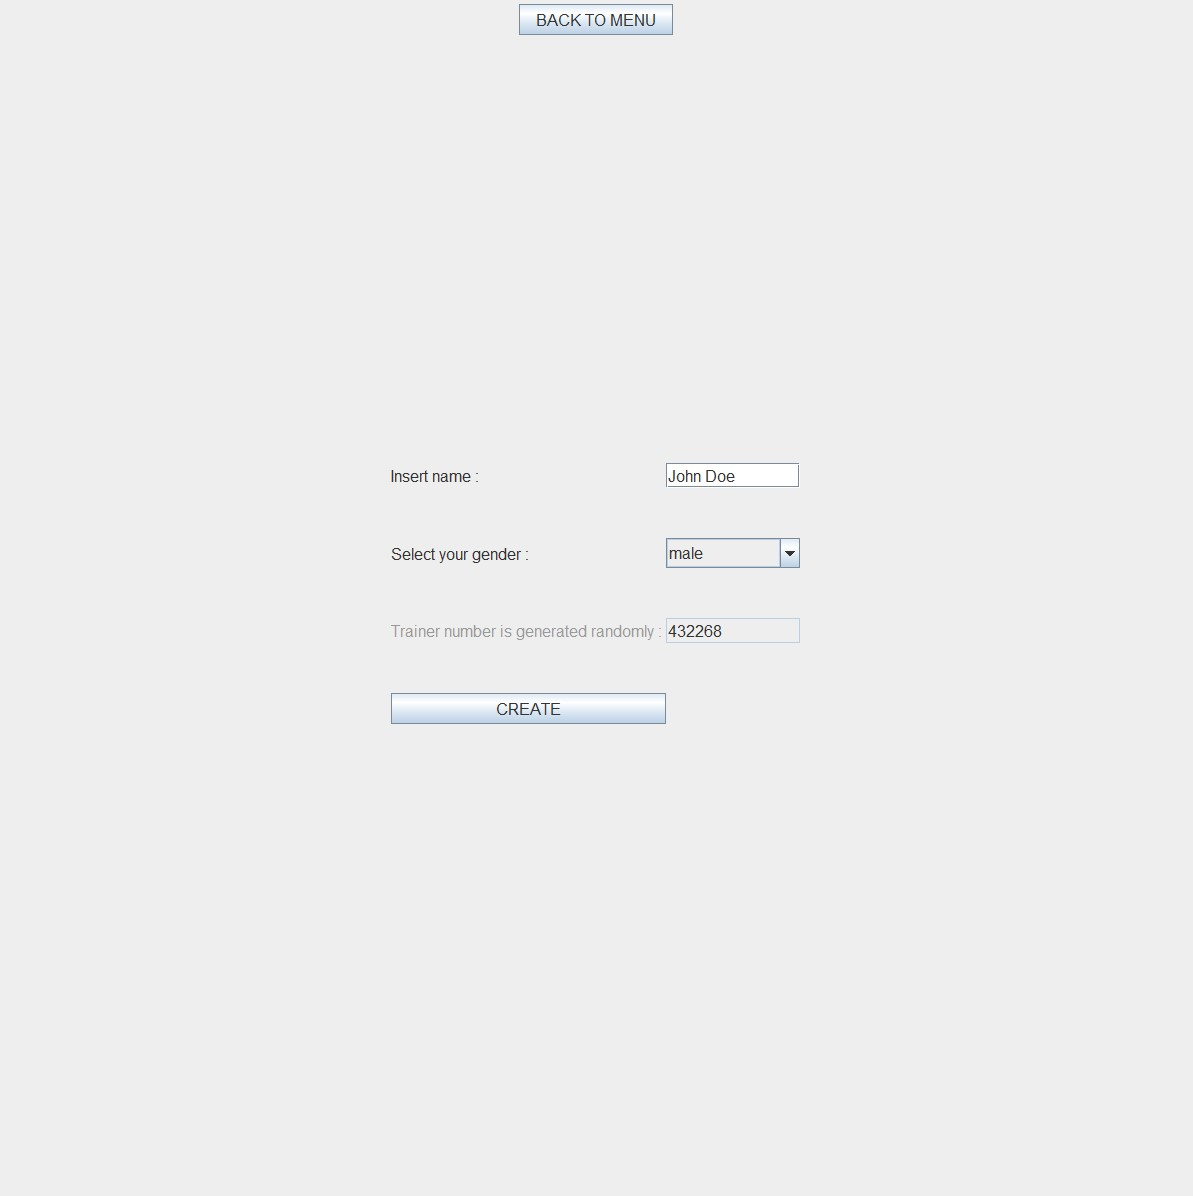
\includegraphics[scale=\x]{Screenshot/start_menu.jpg}
\caption{Menù della creazione di un nuovo personaggio}
\label{img:menu}
\end{figure}

\begin{figure}[H]
\centering
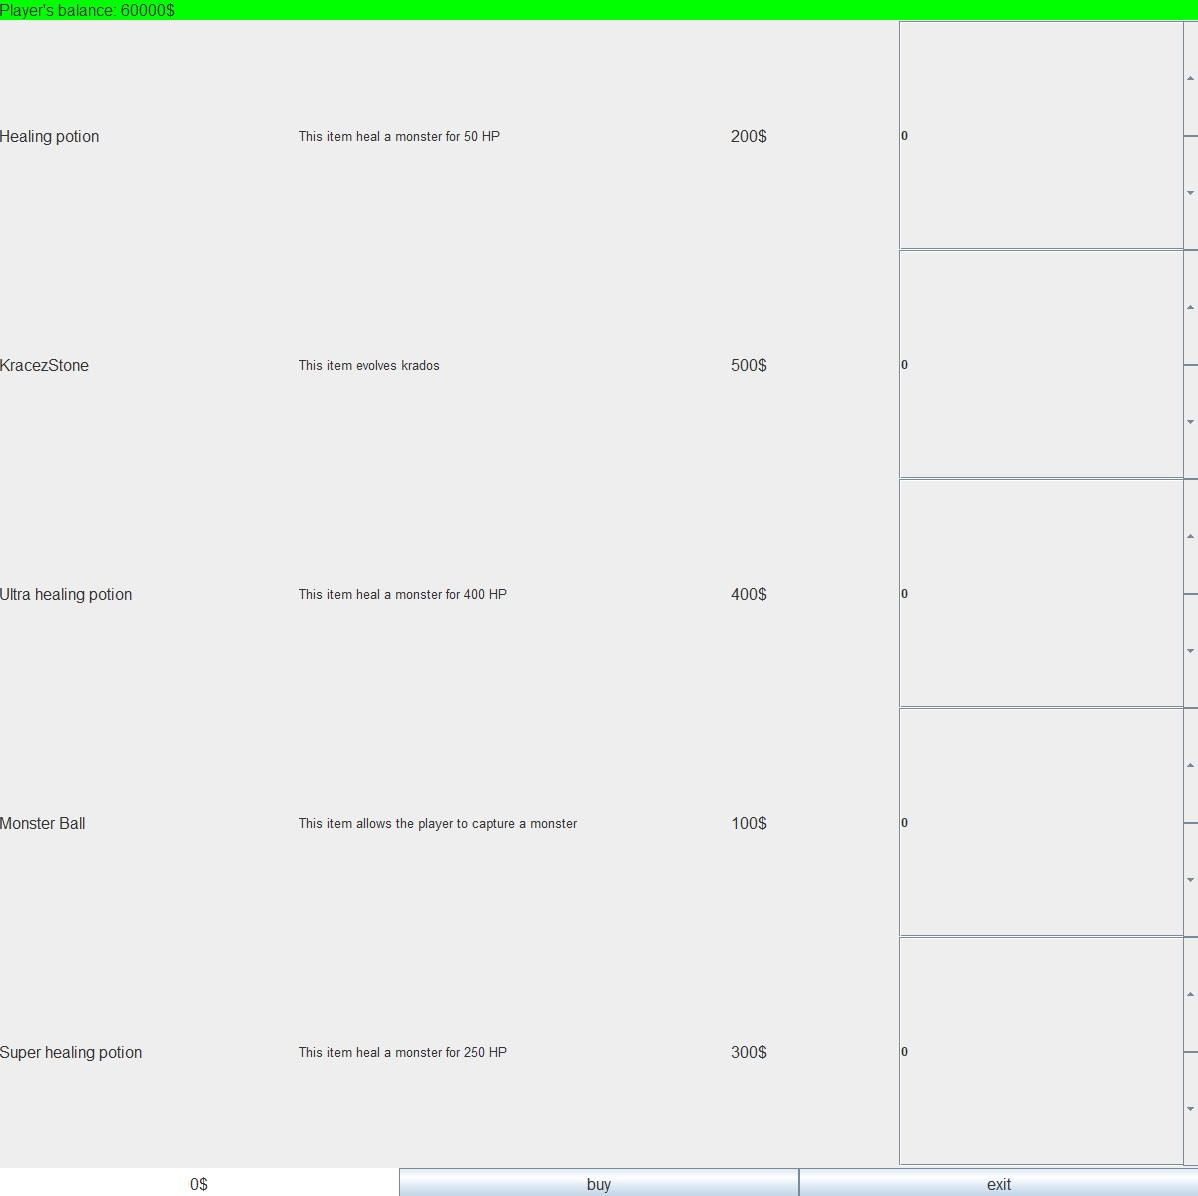
\includegraphics[scale=\x]{Screenshot/merchant.jpg}
\caption{Schermata della vendita degli oggetti}
\label{img:mercante}
\end{figure}

\begin{figure}[H]
\centering
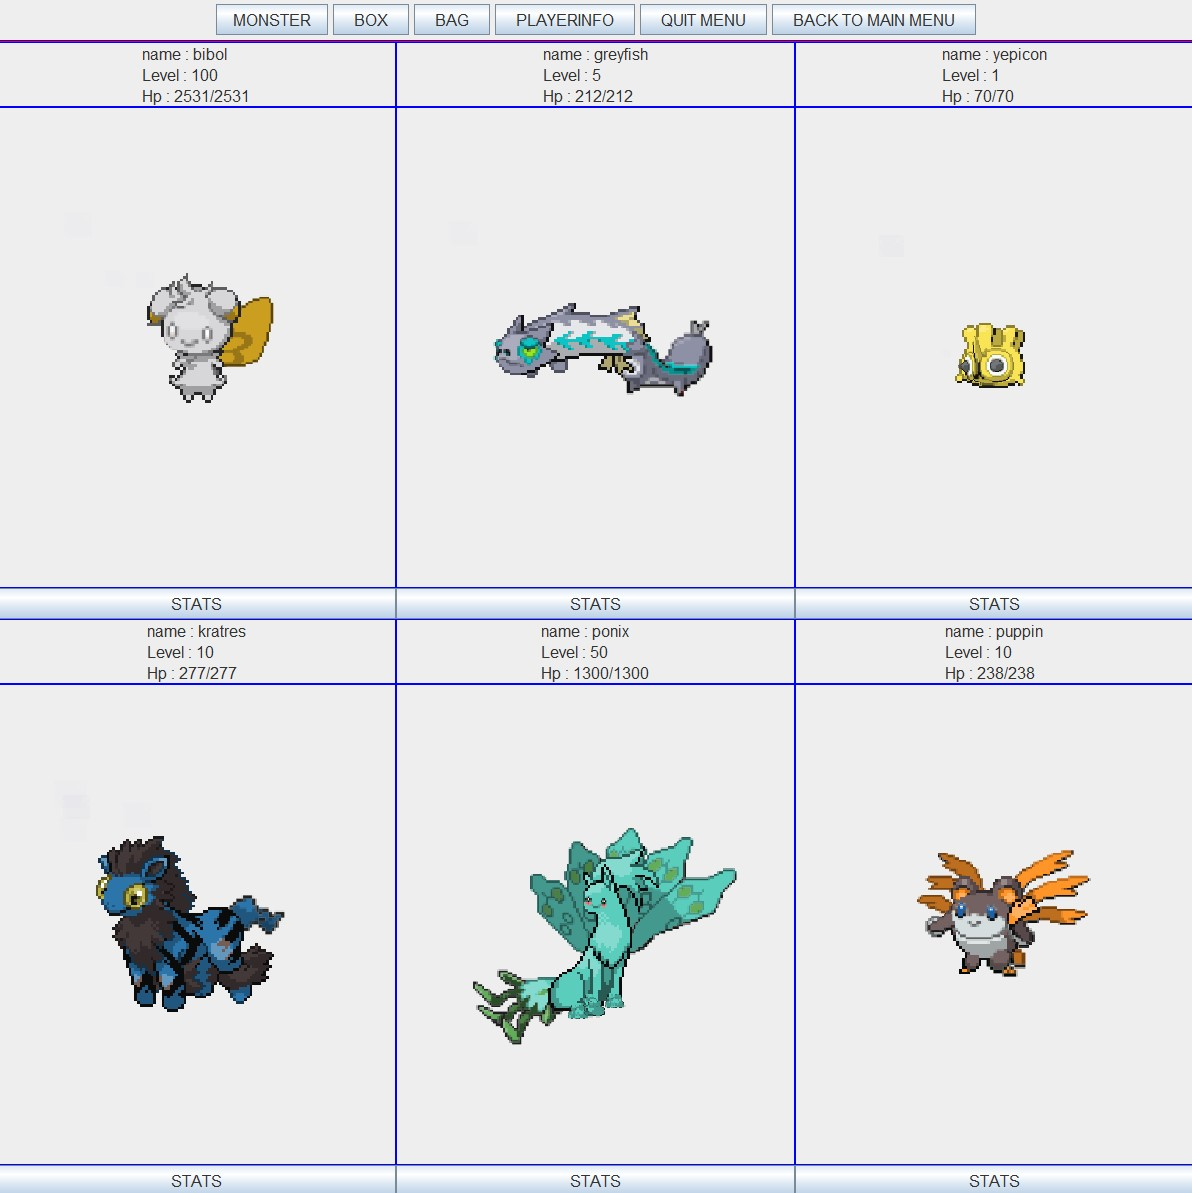
\includegraphics[scale=\x]{Screenshot/inventory.jpg}
\caption{Squadra del giocatore}
\label{img:inventory}
\end{figure}

\begin{figure}[H]
\centering
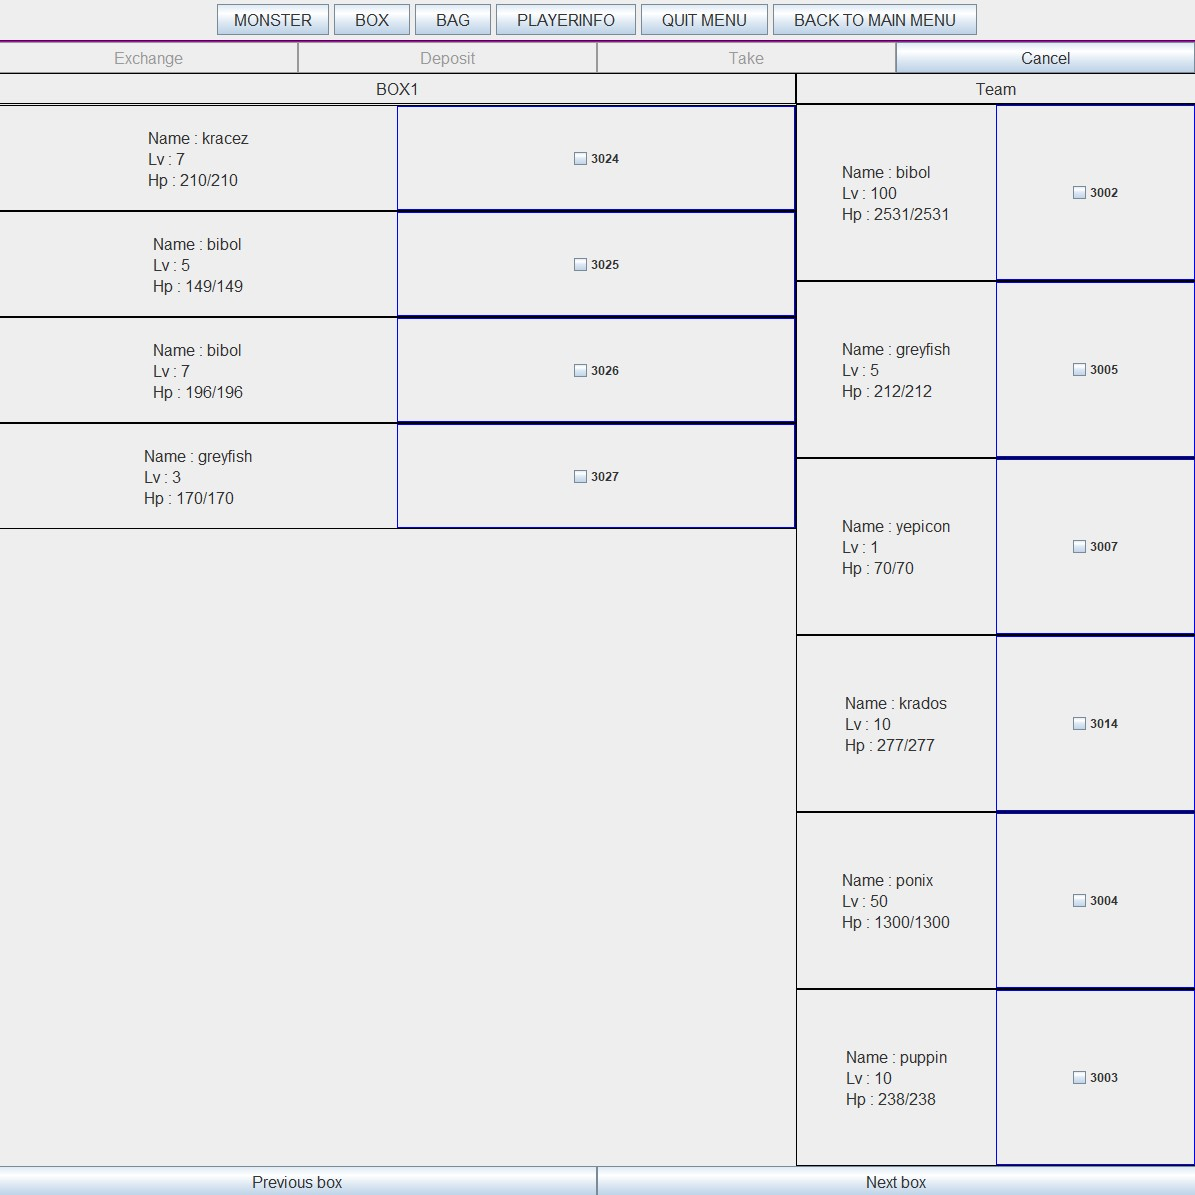
\includegraphics[scale=\x]{Screenshot/storage.jpg}
\caption{Schermata dei box}
\label{img:storage}
\end{figure}


\begin{figure}[H]
\centering
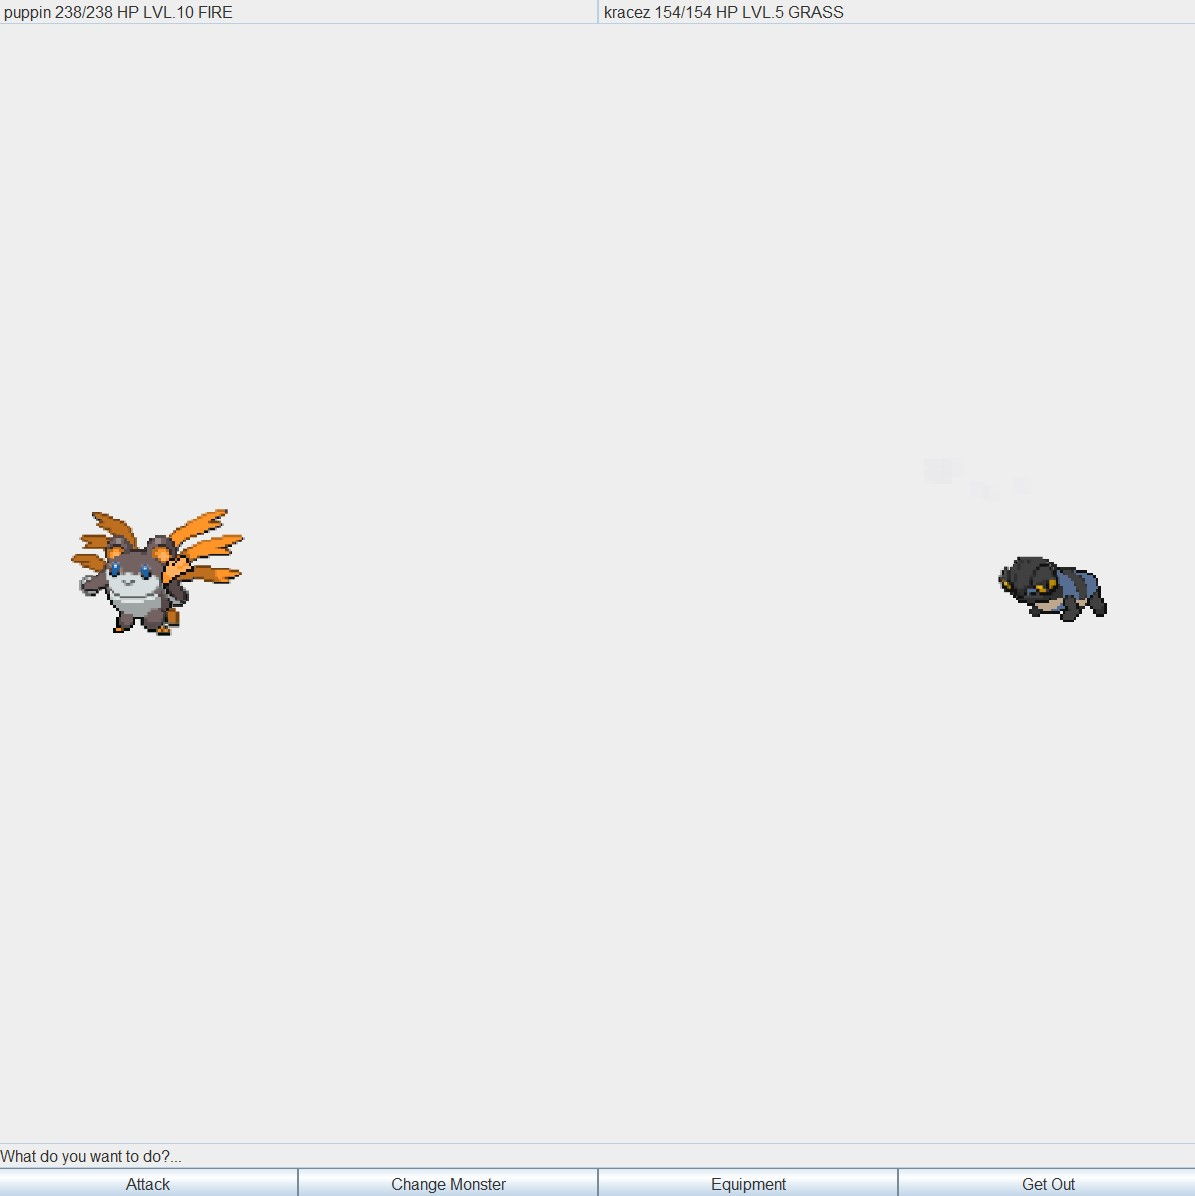
\includegraphics[scale=\x]{Screenshot/battle_panel.jpg}
\caption{Schermata della battaglia}
\label{img:battle}
\end{figure}
